% Compact PGFPlots panel for sampled surface7 BSC bit-scale decomposition.
% Requires \usepackage{pgfplots} and \pgfplotsset{compat=1.18}.
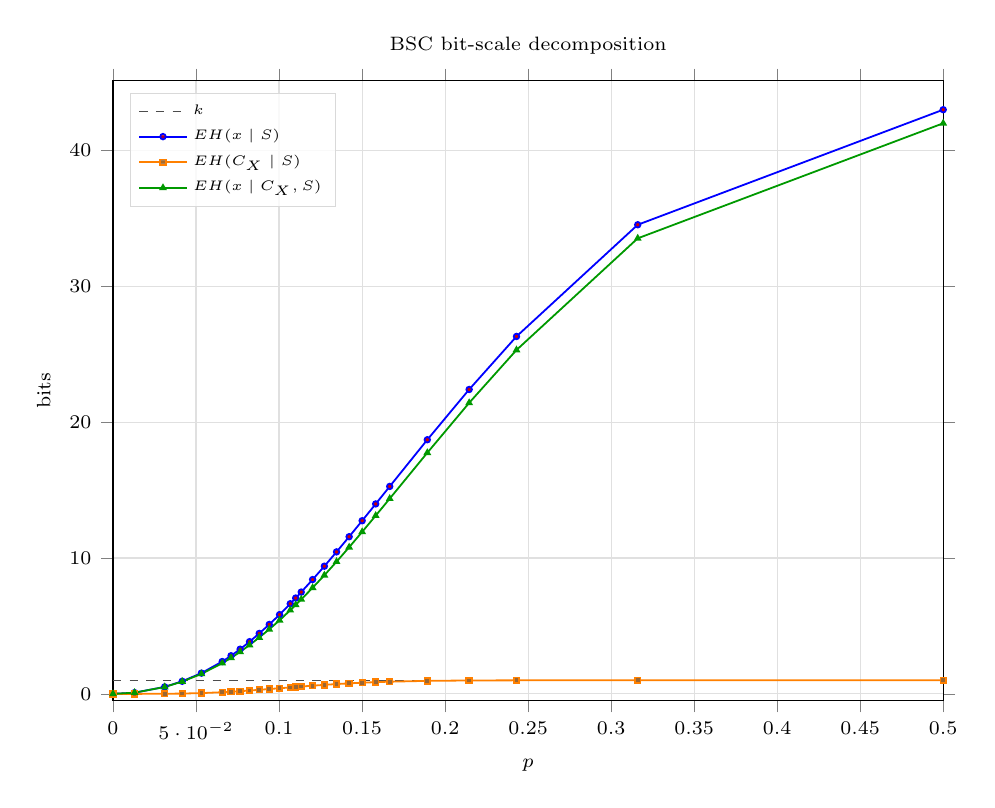
\begin{tikzpicture}
\begin{axis}[
  name=Surface7BSCBitScaleAxis,
  width=\linewidth,
  height=0.78\linewidth,
  title={BSC bit-scale decomposition},
  title style={font=\scriptsize},
  xlabel={$p$},
  ylabel={bits},
  xmin=0, xmax=0.5,
  ymin=-0.5, ymax=45.15,
  grid=both,
  major grid style={black!12},
  minor grid style={black!6},
  tick align=outside,
  tick label style={font=\scriptsize},
  label style={font=\scriptsize},
  legend cell align={left},
  legend style={draw=black!15, fill=white, fill opacity=0.82, text opacity=1, at={(0.02,0.98)}, anchor=north west, font=\tiny},
]
\addplot[black!70, dashed, line width=0.55pt] coordinates {(0,1) (0.5,1)};
\addlegendentry{$k$}
\addplot+[color=blue, mark=*, mark size=1.0pt, line width=0.65pt]
coordinates {(0,0) (0.0129868620555,0.0876698192484) (0.0311244603048,0.513870545668) (0.0416926902737,0.927303910901) (0.0532390407768,1.52780989312) (0.0657867063546,2.37866417308) (0.0710958755299,2.80561636121) (0.0765765344037,3.28841905103) (0.0822333323659,3.84166286502) (0.0880715694979,4.44865996765) (0.0940972433461,5.10873697032) (0.100317108961,5.83212494419) (0.106738753821,6.63247422014) (0.110027864438,7.05460200477) (0.113370689941,7.49351480198) (0.120222466333,8.41339272681) (0.127304805976,9.39855429955) (0.134629772869,10.4504184584) (0.142210976498,11.5677988636) (0.150063823499,12.7450479565) (0.158205829694,13.9810466659) (0.166657010397,15.2693392603) (0.189297705371,18.7062483776) (0.21450174486,22.4069169196) (0.243003853809,26.3080933385) (0.316019346324,34.5308907941) (0.5,43)};
\addlegendentry{$\mathbb{E}H(x\mid S)$}
\addplot+[color=orange, mark=square*, mark size=1.0pt, line width=0.65pt]
coordinates {(0,0) (0.0129868620555,8.51418994291e-05) (0.0311244603048,0.00746801320557) (0.0416926902737,0.0234311846593) (0.0532390407768,0.0569426791414) (0.0657867063546,0.121069652832) (0.0710958755299,0.157063521277) (0.0765765344037,0.198763517594) (0.0822333323659,0.24607305196) (0.0880715694979,0.299318081958) (0.0940972433461,0.356455800008) (0.100317108961,0.415003068084) (0.106738753821,0.474176791317) (0.110027864438,0.507627725604) (0.113370689941,0.540418579351) (0.120222466333,0.602809092295) (0.127304805976,0.665427008459) (0.134629772869,0.721851407122) (0.142210976498,0.774318484135) (0.150063823499,0.821148801923) (0.158205829694,0.862513770917) (0.166657010397,0.897126325537) (0.189297705371,0.957621361284) (0.21450174486,0.986164115221) (0.243003853809,0.996610973702) (0.316019346324,0.999936375875) (0.5,1)};
\addlegendentry{$\mathbb{E}H(C_X\mid S)$}
\addplot+[color=green!60!black, mark=triangle*, mark size=1.0pt, line width=0.65pt]
coordinates {(0,0) (0.0129868620555,0.087584677349) (0.0311244603048,0.506402532462) (0.0416926902737,0.903872726242) (0.0532390407768,1.47086721398) (0.0657867063546,2.25759452025) (0.0710958755299,2.64855283993) (0.0765765344037,3.08965553344) (0.0822333323659,3.59558981306) (0.0880715694979,4.14934188569) (0.0940972433461,4.75228117031) (0.100317108961,5.4171218761) (0.106738753821,6.15829742882) (0.110027864438,6.54697427917) (0.113370689941,6.95309622262) (0.120222466333,7.81058363451) (0.127304805976,8.73312729109) (0.134629772869,9.72856705129) (0.142210976498,10.7934803795) (0.150063823499,11.9238991545) (0.158205829694,13.118532895) (0.166657010397,14.3722129347) (0.189297705371,17.7486270163) (0.21450174486,21.4207528044) (0.243003853809,25.3114823648) (0.316019346324,33.5309544182) (0.5,42)};
\addlegendentry{$\mathbb{E}H(x\mid C_X,S)$}
\end{axis}
\end{tikzpicture}
